\chapter{Formulácia problému a riešenie}

\section{Formulácia problému}
\par{
Pojem Digitálne dvojča (DT) sa čoraz častejšie využíva ako nástroj na modelovanie, navrhovanie a prototypovanie \cite{dt-iot}. V rámci 5G technológie ide o presnú digitálnu repliku siete, ktorá si s reálnou sieťou vymieňa dáta obojsmerne, v reálnom čase, v snahe zlepšiť manažment siete či zrýchliť vývoj 5G sietí \cite{systematicReview}.
}
\par{
Hoci 5G siete ponúkajú nízku latenciu a vysokú rýchlosť, sú limitované v predikcii správania, a to pre dynamiku používateľov, zaťaženie či zmeny prostredia \cite{dt-network}. DT by mohlo tieto výzvy prekonať predpoveďami budúceho stavu siete, čím by na základe aktuálneho zaťaženia siete umožnilo dynamické riadenie alokácie zdrojov a zlepšilo celkovú výkonnosť systému\cite{5g-challenges}.
\\ 
Zásadnú výzvu predstavuje práca s veľkým objemom dát, v reálnom čase, ktorá si vyžaduje vysokú výpočtovú silu, zaťažujúcu hardvér \cite{challenges-technol} a rovnako tak zachovanie nízkej latencie pri dosahovaní vysokej presnosti simulácie, potrebnej na predikciu budúceho stavu siete. Samotný model a konfigurácia DT predstavujú časovo a implementačne komplexné časti spomínaného riešenia \cite{challengesAndApplicationsReview}.
}

\section{Technický literárny prehľad}
\par{
Pojem digitálneho dvojčaťa sa v posledných rokoch, predovšetkým v technických oblastiach, spomína stále častejšie. Vzhľadom na digitalizáciu, ktorá je prítomná v každom sektore, sa transformácia hmatateľného sveta do sveta bitov a pixelov stáva prirodzeným výsledkom tohto trendu. 
}
\par{
V technickej literatúre sa DT definuje ako virtuálna reprezentácia fyzického objektu, medzi ktorými prebieha bilaterálny tok dát v reálnom čase \cite{DT:OriginToFuture}. Tok dát zabezpečuje presné zrkadlenie správania oboch týchto entít \cite{systematicReview}. Vlastnosť zrkadlenia poskytuje možnosti preventívnej údržby, či navrhovania ďalších generácií biznis modelov \cite{5g&beyond}.
}

\begin{figure}[H]
    \centering
    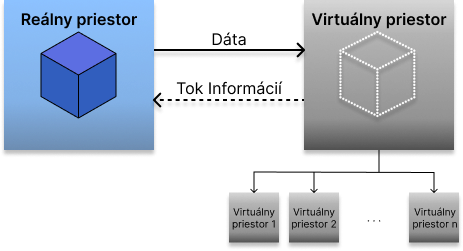
\includegraphics[width=0.85\linewidth]{assets/images/Grieves_PLM_model.png}
    \caption{Digitálne dvojča}
\end{figure}

\par{Vo  svojom výskume Enders a Hoßbachová \cite{DimensionOfDTAplication} identifikovali sektory, kde je používanie digitálneho dvojčaťa najrozšírenejšie. Patria sem výroba, letecký priemysel, energetika, automobilový priemysel, námorníctvo, petrochemický priemysel, poľnohospodárstvo, zdravotníctvo, verejný sektor a ťažba.
}
\par{Taktiež identifikovali tri hlavné využitia digitálneho dvojčaťa v týchto oblastiach: ovládanie, simulovanie a monitorovanie. To však ani zďaleka nepokrýva všetky možnosti a spôsoby využitia. Digitálne dvojča dnes nájde uplatnenie aj pri dizajnovaní, validácii, predchádzaní chýb, trénovaní, optimalizácii a predikcii \cite{AplicationsOfDT}.
}
\par{Ak sa chceme pozrieť na reálne aplikácie DT, Huawei implementoval DT na monitorovanie výrobných liniek \cite{huawei2020}, zatiaľ čo mestá ako Bristol \cite{Bristol} či Singapur \cite{singapur} používajú DT na efektívne riadenie inteligentných mestských systémov. V týchto scenároch DT umožňuje predikciu zlyhaní, optimalizáciu zdrojov a minimalizáciu prestojov. Podobné prístupy sú použiteľné aj v telekomunikáciách, kde DT dokáže simulovať a predikovať správanie sietí v reálnom čase. 
}
\par{V oblasti telekomunikácií sa čoraz viac využívajú pri simuláciách rádiových prístupových sietí (RAN), monitorovaní jadra siete a optimalizácii zdrojov. Napríklad Siemens nasadzuje DT na správu a optimalizáciu sieťových komponentov \cite{5g&beyond}. Podobne, ZTE a China Mobile úspešne aplikovali technológiu digitálneho dvojčaťa na zlepšenie 5G konektivity pre vysokorýchlostnú železničnú trať v južnej Číne. Pomocou presného 3D modelu infraštruktúry popri trati optimalizovali výkonnosť 5G siete, čím dosiahli pokrytie na úrovni 98,5\% a rýchlosti sťahovania presahujúce 300 Mbps \cite{ChinaMobile}. 
}
\par{ Tieto úspešné implementácie demonštrujú širokú škálu výhod technológie DT v telekomunikáciách, od optimalizácie pokrytia po zvyšovanie kvality služieb. Napriek tomu však existujú určité obmedzenia, ako napríklad zložitosť nasadenia, škálovateľnosť a presnosť simulácií, ktoré je potrebné prekonať pri vývoji nových riešení. 
}

\section{Prehľad riešenia (na vysokej úrovni)}
\par{
High level = denoting a programming language that is relatively accessible to the user, having instructions that resemble a natural language such as English.
}
\\ 
par{
Stručne vysvetlite riešenie problému. Študenti by mali byť schopní odôvodniť svoj výber techník použitých na riešenie problému, uznať ich obmedzenia a interdisciplinárny dosah. | 2-3 strany
}
Nástroje a prístupy:  \\
- rôzne nástroje na tvorbu a správu DT (ansys, matlib a simulink ...)
- nástroje pre 5G:
    - srsRAN: Open-source - radio network simulation.
    - Open5GS: 5G core network.
    - UERANSIM: user equipment (UE) and radio access networks (RAN).
Prečo práve tieto nástroje?
\par{
Návrh riešenia - High Level \\
- overview môjho spôsobu riešenia pre 5G DT
- ako bude DT napodobňovať reálnu sieť? - real-time data, pozorovania a predikcie stavov, ktoré budú nasledovať

Výber technológií: \\
Prečo práve srsRAN pre Radio Access Network (RAN) [Allows RAN simulation, offering control over radio settings, configurations.], 
Open5GS pre core network [Provides core network functions for handling control and user plane traffic.], 
a UERANSIM pre simulácie user devices a scenarios[Generates realistic device traffic, lets you test a range of scenarios.].

Architektúra - návrh: \\
- Diagramy alebo popísané komponenty:
Network core (Open5GS).
Radio Access Network (srsRAN).
Simulated User Devices (UERANSIM).
- Flow dát medzi nimi: \\
srsRAN a Open5GS komunikujú, a ako UERANSIM interaguje s RAN aa core network pre simulovanie real-world trafficu.

Data flow a predikcia: \\
- (potrebujem vedieť aké dáta dokážeme vyťiahnuť zo srsRAN Project) (latency, bandwidth usage, packet loss)
- Aký je plán implementácie predikčného modelu (ML) aké stavy bude mať učenie, aký preprocessing dát ... 


Limitácie: \\
- presnosť, computational load
- hw limitácie
- časové limitácie
- programové limitácie simulinku a matlabu ak nejaké budú
}

\section{Hodnotenie rizík}
\par{
Implementácia digitálneho dvojčaťa 5G siete spolu s modelom ML prináša rôzne výzvy, ktoré môžu ovplyvniť presnosť predpovedí, stabilitu a efektívnosť celého systému. Identifikácia týchto problémov a návrh stratégií na ich zmiernenie sú jednou z kľúčových úloh tejto práce.

Nedostatočná kvalita vstupných dát je jedným z najpravdepodobnejších rizík, ktoré môžu viesť k nesprávnym výsledkom modelu. Chyby v dátach alebo ich nereprezentatívnosť, napríklad pri modeloch sieťovej prevádzky (traffic patterns), môžu narušiť presnosť predpovedí \cite{ML_traffic}. Formou zmiernenia je testovanie na rôznych dátových scenároch a aplikácia metód ako krížová validácia a ladenie hyperparametrov, ktoré minimalizujú riziko chýb spojených s podtrénovaním (underfitting) a pretrénovaním (overfitting) \cite{Nguyen}.

Zber kvalitných dát môže byť problematický, pretože mnohé scenáre je potrebné zachytiť v laboratóriu. Bez dostatočných dát môže model generovať neadekvátne predpovede, ktoré nebudé reprezentovať skutočnosť. Riešením môže byť generovanie syntetických údajov \cite{data_generating} a využitie dostupných datasetov z iných projektov \cite{datasets_telecom}, ktoré môžu čiastočne nahradiť reálne dáta a napomôcť k presnejším predpovediam.

Nezvyčajné scenáre, ako vysoké zaťaženie siete (peak loads), neštandardné správanie používateľov či poveternostné podmienky môžu narušiť schopnosť modelu adaptovať sa \cite{challenges_human_factor}. Ak tieto scenáre neobsahujú trénovacie dáta, model nemusí byť pripravený na takéto situácie. Vzhľadom na čas, ktorý máme na získanie a predspracovanie dát, tento problém nemusí byť vo finálnej implementácií vyriešený dostatočne, a preto jeho vyriešenie vyžaduje ďalšiu prácu a zber dát.

Kompatibilita systémov ako srsRAN, Open5GS, UERANSIM a nástrojov Docker nie je vždy automatizovaná, čo môže ovplyvniť celkovú integráciu práce \cite{challenges_human_factor}. Pre zváladnutie tohoto problému sa implementácia začína na malých izolovaných komponentoch, pričom ich spolupráca sa testuje krok za krokom. Takéto testovanie, a celkový vývoj DT je časovo veľmi náročné, čo potvrdili aj autori v \cite{USAirForce}. Tento fakt môže negatívne vplývať na výsledok celej práce.

Konfigurácia siete môže odhaliť citlivé informácie o 5G infraštruktúre či porušenie GDPR \cite{big-data-problems} pri nechcenom zachytení údajov o používateľoch \cite{challenges-technol}. Únik takýchto dát by ohrozil nielen bezpečnosť projektu, ale aj reálnej siete \cite{Dt_Iot_data_worry_about}. Používanie .env súborov na uchovávanie citlivých premenných a simulovanie siete s fiktívnymi údajmi výrazne znižuje riziko úniku.
}

%\par{Študenti by mali rozpoznať riziká spojené s implementáciou ich riešení a ponúknuť stratégie na ich zmiernenie. | max. 1 strana}

\begin{comment}
\section{Experimentálna reprodukovateľnosť a integrácia}
\par{
Fáza inžinierstva riešení by mala byť vykonávaná s ohľadom na reprodukovateľnosť a systémovú integráciu a študenti by mali podrobne opísať, ako sa tejto otázke venovali. Pokiaľ nie sú špeciálne podmienky, kód, modely a dáta použité pri inžinierstve riešení by mali byť voľne dostupné. Modely strojového učenia by mali byť prezentované tak, aby umožňovali ďalšie využitie bez nutnosti rekvalifikácie. Tam, kde je to možné, použite riešenia v kontajneroch, ktoré zabezpečia použiteľnosť produktu alebo služby aj pri zmene základnej technológie. | 3 strany
}
\par{
Setup Documentation: \\
- step-by-step instalacia na jednotlivých VMs
- neviem či sa bude dať docker (?) - ale pravdepodobne aspoň na niečo by sa dalo - setupy VMs a resp, celé VM dať do dockeru

Source Code - dostupnosť: \\
GitHub - Readme, version control

Úvahy o integrácií: \\
- Modularita komponentov - každý z nich má svoju funkciu a umožňuje rozširovanie
Logovanie a Interface konzistencia: \\
- popisať ako logujeme data, aby to bolo reprodukovateľné

Future-Proofing: \\
- izolovanie komponentov, mozne zmeny bez nutnosti meniť celý projekt

Machine Learning a znovu použiteľnosť:\\ 
- Popísať ako je model trenovaný, aká je jeho architektúra, parametre a hyperparametre + trénovacie dáta
- zabezpečiť, aby bol už model natrénovaný, aby ho ostatní v budúcnosti nemuseli trénovať znova.
- spomenúť knižnice, štandardy
}
\end{comment}


%Študenti by mali opísať, ako by implementovali opatrenia na zabezpečenie udržateľnosti svojho produktu alebo služby počas životného cyklu. | 1-2 strany
\section{Udržateľnosť a environmentálny dopad}
\par{
Implementácia opatrení na zabezpečenie udržateľnosť projektu a minimalizácia jeho environmentálneho dopadu sú kľúčové pre zaistenie dlhodobej hodnoty, spoločenského prínosu a efektivity vypracovania tejto práce. Práca je navrhnutá s dôrazom na efektívne využívanie zdrojov, udržateľný softvérový a hardvérový návrh a životný cyklus, ktorý minimalizuje potrebu fyzických zdrojov.
}

\par{
Jednou z hlavných prínosov DT je možnosť predikcie a optimalizácie, čo vedie k redukcii využívania zdrojov. Predikcia záťaže siete umožňuje lepšiu správu záťaže (traffic load) a preťaženia (congestion), čo znižuje potrebu nadmernej spotreby energie. Optimalizácia smerovania (routing) prispieva k zlepšeniu celkovej efektivity siete. Navyše, digitálne dvojča eliminuje potrebu testovania na fyzických zariadeniach, čím sa minimalizuje spotreba elektrickej energie, rôznych materiálov a času potrebného na fyzické experimenty. Tento prístup je obzvlášť užitočný v prípade nasadzovania 5G technológií v oblastiach s obmedzenými zdrojmi.
}

\par{
Vývoj softvéru bol orientovaný na maximálnu efektivitu, čo zahŕňa optimalizáciu kódu na zniženie spotreby energie počas behu aplikácie a nasadenie projektu v prostredí Docker, čo umožňuje efektívnejšiu konfiguráciu a škálovateľnosť strojov. Tieto opatrenia nielen znižujú environmentálny dopad, ale aj zlepšujú celkovú udržateľnosť projektu.
}

\par{
Modulárny dizajn projektu zaisťuje, že aktualizácie a údržba nemajú vplyv na celkovú funkčnosť systému. Tento prístup znižuje potrebu kompletného prekonfigurovania alebo fyzických zásahov, čo prispieva k dlhodobej udržateľnosti.
}

\par{
Použitie prediktívnych modelov v digitálnom dvojčati vedie k zásadným environmentálnym prínosom, ako je znížené zaťaženie fyzickej infraštruktúry a menej časté aktualizácie fyzického hardvéru, čo vedie k nižšej spotrebe zdrojov a menšej produkcii odpadu. Predikčné modely teda umožňujú efektívnejšie rozhodovanie s pozitívnym dopadom na životné prostredie.
}



\begin{comment}
Zdroje:
https://www.mdpi.com/2072-4292/14/6/1335#B80-remotesensing-14-01335
https://www.mdpi.com/2076-3417/11/12/5519
https://www.mdpi.com/1424-8220/23/16/7262
https://www.europarl.europa.eu/RegData/etudes/STUD/2021/690021/EPRS_STU(2021)690021_EN.pdf
https://ietresearch.onlinelibrary.wiley.com/doi/full/10.1049/dgt2.12008
https://www.mdpi.com/1996-1073/14/7/1885

Resource Efficiency: \\
- predikcia -> redukcia wasteful používanie zdrojov
- zmena traffic routingu, lepšia správa traffic loadu a congestion
- zníženie power (energy) consumption

- máme DT tak nemusíme testovať fyzické zariadenia a reálnu energiu (el., čas) - využitie ak sa má 5G dostať do oblastí, kde nie sú zatiaľ všetky resources -> zistíme popredu či sa tam oplatí ísť [nie priamo moja práca ale celkovo 5G DT]

Sustainable Software:\\
- kód, ktorý bude čo najefektívnejší, menšia power consumption
- ak to bude bežať v dockeri tak to zefektívni nastavovanie strojov

Lifecycle Management: \\
- modularita zabezpečuje, že aktualizáie a údržba nezastavia celý systém a nemusíme všetko nastavovať odzačiatku

Environmentálne Benefits predikovania: \\
- znížené zaťaženie infraštruktúry a menej časté aktualizácie fyzického hardvéru, čo vedie k nižšej spotrebe zdrojov..
\end{comment}

\section{Zamestnateľnosť}
\par{
Táto bakalárska práca, zameraná na rozvoj teoretických znalostí v oblasti digitálnych dvojčiat v spojení s praktickou implementáciou a optimalizáciou 5G sietí, má veľký potenciál rozšíriť zručnosti vo viacerých kľúčových oblastiach technologického sektora. V neposlednom rade strojové učenie, použité na predikciu správania implementovaného digitálneho dvojčaťa, zasahuje aj do oblasti dátovej vedy.

Vďaka formátu práce autori prejdú celým cyklom realizácie projektu, od prieskumu technológií cez návrh až po implementáciu a testovanie. Týmto získajú ucelený a komplexný pohľad na vývoj a riadenie softvérových projektov, ako aj na plánovanie, organizáciu a efektívnu komunikáciu.

Takáto kombinácia technických, projektových a komunikačných schopností môže významne zvýšiť hodnotu autorov na trhu práce, najmä v budúcnosti, keďže problematika digitálnych dvojčiat a 5G sietí je stále viac žiadaná a nachádza uplatnenie v rôznych odvetviach.
}\begin{comment}
\section{Tímová práca, diverzita a inklúzia}
\par{
Ak sa na projekte podieľajú odborníci z viacerých odborov, študent by mal implementovať procesy a opísať techniky pre zdieľanie úloh a (pochopenie) znalostí medzi rôznymi stranami. Mali by sa opísať problémy a stratégie na ich zmiernenie, aby sa zabezpečilo dokončenie projektu v stanovenom časovom harmonograme. Táto časť by mala obsahovať aj úvahy o diverzite a inklúzii. | ½-1 strana
}
\par{
Teamwork and Knowledge Sharing: \\
- spolupráca s Matejom a Matejom

Diversity and Inclusion:
- Ageism - pomoc pre všetky vekové skupiny?
- Disabled people? hearing, vision ...
- môže im to DT nejko pomôcť?
- Prehľadná dokumentáia a návod pre možnú spoloprácu...
}

Spolupráca s konzultantom a inými odborníkmi: Môžete zdôrazniť, ako ste spolupracovali s konzultantom, odborníkmi alebo kolegami, aby ste získali spätnú väzbu alebo konzultovali technické aspekty projektu.

Diverzia myšlienok a prístupov: Aj keď ste projekt riešili individuálne, môžete opísať, ako ste zohľadnili rôzne perspektívy pri výbere riešení a metodík. Napríklad môžete zdôrazniť, že ste čerpali z rôznych zdrojov, ako sú články, výskumy a prípadové štúdie, aby ste vytvorili univerzálne použiteľný a inkluzívny návrh.

Prístupnosť a inklúzia výsledkov projektu: Opíšte, ako váš projekt môže byť prínosný pre širšiu komunitu používateľov. Napríklad, ak je váš digitálny dvojča schopné zlepšiť efektivitu nasadzovania 5G sietí, môže byť relevantný aj pre menej rozvinuté regióny alebo oblasti so zníženými zdrojmi.

Schopnosť prispôsobiť projekt tímovému pracovnému prostrediu: Môžete uviesť, že ste navrhli systém s ohľadom na modularitu a jednoduchú integráciu, čo umožňuje budúcu spoluprácu tímov na rozšírení projektu

Článok - Intro a Related work
\end{comment}